
Consider a tracking crime application where civilians and police share information about criminality in given zones of a city. 
Civilian users signal crimes using Twitter.
Police officers can notify crimes, as well as update information about solving cases.
Some of these information are confidential while other can be shared
to the community of users using this application. 

Users can track crimes in given zones. 
Crime information stored by the system may be visualized on a map. 
Some users have different access rights than others.
For example, police officers have more access rights than civilians.


In order to provide these functionalities, the application uses pre-existing services to provide, store and visualize the information.
The business process defines the logic of the application and is specified in terms of tasks. 
Tasks can be performed by persons or computers. 

The business process and requirements specifications presented in Figure~\ref{fig:constraints} are instances of the Computation-Independent models of Figure~\ref{fig:piSOD-M}.
Busines process is represented as a graph while requirements are given as text boxes.
\begin{figure}[ht!]
\centering
%\subfloat[\textit{Tracking Crimes} - Illustration of the Problem.]
%{\label{fig:problem}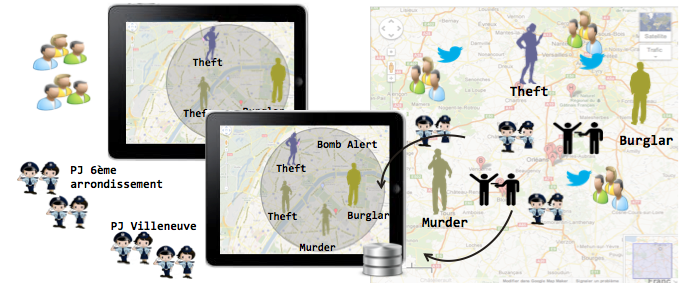
\includegraphics[width=0.95\textwidth]{figs/problem}}
%~ %add desired spacing between images, e. g. ~, \quad, \qquad etc. (or a blank line to force the subfig onto a new line)
%\\
%\subfloat[Contraints.]
{\label{fig:trans06}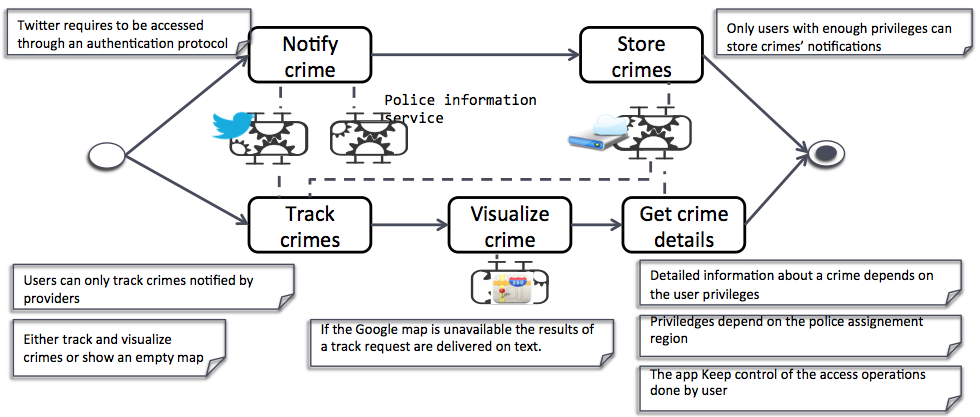
\includegraphics[width=0.95\textwidth]{figs/constraints}}
~ %add desired spacing between images, e. g. ~, \quad, \qquad etc. (or a blank line to force the subfig onto a new line)
\caption{Business process for the tracking crime example.}
\label{fig:constraints}
\end{figure}

In our example, crime processing can start with one of two tasks: \textit{(i) notify a crime}, or \textit{(ii) track a crime}.
Notified crimes are stored in a database. 
Tracked crimes are visualized in a map.
The used can ask for detailed information. 
The application is built upon four services: \textsf{twitter} and an \textsf{ad-hoc police service} for notifying crimes, \textsf{Amazon} used as  persistence service and  \textsf{Google Maps} for locating and displaying crimes on a map.

Non-functional requirements are specified by rules and conditions to be verified during the excecution of tasks.
In our example we have the following non-functional requirements:
\begin{trivlist}
\item[1.] Twitter requires to be accessed through an authentication protocol that allows three login failures before blocking. 
\item[2.] Crime notification needs privileged access.
\item[3.] Civilian users can only track crimes for which they have clearance: Civilian population cannot track all the crimes notified by the police. 
\item[4.] If \textsf{Google Maps} is unavailable, the results are delivered as text. 
\item[5.] Querying about crimes without having proper clearance yields an empty map.
\item[6.] Access rights to detailed information depends on user clearance and zone assignment for police officers. 
\item[7.] The application maintains a detailed log. 
\end{trivlist}

Considering the example of tracking crimes, all the system restrictions are
model as constraints in the methodology. We have three types of constraints:
\textit{value}, \textit{business} and \textit{exceptions behaviour} constraints.
Each use case can be associated to one or more constraints.

\paragraph*{\textit{$\pi$-UseCase} model:} 
In our example we have five use cases (Figure~\ref{fig:piUC}), which represent the
system functions (tasks) and constraints. 
We will not detail the functional part of the specification, due to lack of space.
The constrains defined for our tracking crime example are: 

\begin{trivlist}
  \item[-] The \textsf{Notify crime} task requires that the user is logged in. 
  This is an example of a \textit{value constraint}, where the value associated to the condition depends on the semantics of the application.
  In this case, it represents the maximmum number of allowed login attempts;
\item[-] The \textsf{Store crimes} task requires the verification of the user's clearance (also a value constraint). 
\item[-] In order to perform the \textsf{Track crimes} task, it is necessary that the notifier user is in the contact list of the requesting user.
This is an example of \textit{business constraint}.
Additionally the requesting user must be logged in.
\item[-]  For the \textsf{View Crime Map} task, the specification defines that if the Google Maps service is not available, the result is presented as text. This is an example of \textit{exceptional behaviour constraint}. 
The availability of the Google Maps service is verified by a \textit{business constraint}.
 \item[-] The \textsf{Show crime details} task is specified to have three constraints: A \textit{value constraint} is defined to verify the user's clearance level; A \textit{business constraint} is used to ensure that the user's clearance is valid for the geographic zone of the crime; Another \textit{value constraint} defines that the log is to be maintained.
\end{trivlist}
\begin{figure}[ht!]
\centering
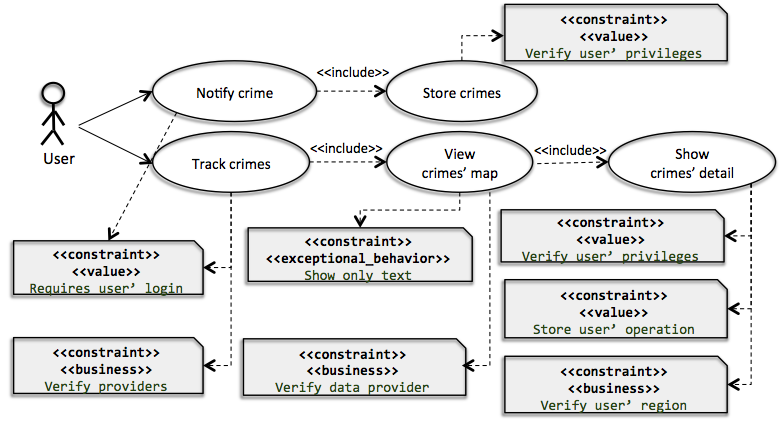
\includegraphics[width=0.8\textwidth]{figs/piUseCase}
\caption{$\pi$-UseCase Model}
\label{fig:piUC}
\end{figure}
\paragraph*{\textit{$\pi$-ServiceProcess} model:}
The model presented in Figure~\ref{fig:piUC} is transformed, at this stage of the development, into a similar graph, where \textit{(i)} the task nodes are better detailed, by refining the control and data flows; and \textit{(ii)} constraints are transformed into \textit{contracts} (pre- and post-conditions).
The new model describes the application's activities and defines contracts for each activity or for parts of the application.

A model-to model transformation is defined in order refine the \textit{$\pi$-UseCase} model of the application into the more detailed model. 
This (semi-automatic) transformation process is supported by a tool (described in~\cite{SouzaNeto:2012}).

The \textit{$\pi$-ServiceProcess} model defined for our tracking crime application is presented in Figure~\ref{fig:piSP}, where: 
\begin{enumerate}
\item Tasks of the previous model are transformed into \textit{actions};
\item Actions are grouped into \textit{activities} (in accordance to the business logic).
\item Constraints of the \textit{$\pi$-UseCase} model are transformed into assertions.
\end{enumerate}

\begin{figure}[ht!]
\centering
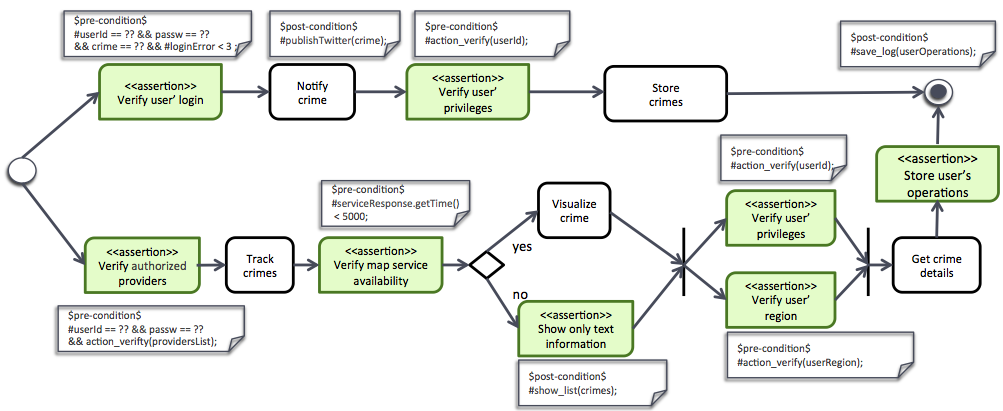
\includegraphics[width=0.99\textwidth]{figs/piServiceProcess}
\caption{$\pi$-\textit{ServiceProcess} Model}
\label{fig:piSP}
\end{figure}

\paragraph*{\textit{$\pi$-ServiceComposition} model:} 
This model refines the previous model by using the activities to produce the workflow of the application.
The model serves to identify those entities that collaborate with the service process by providing services to execute actions. 
This model identifies the services and functions that correspond to each action in the business process.

\begin{figure}[t]
\centering
\subfloat[$\pi$-ServiceComposition Model]
{\label{fig:piSC}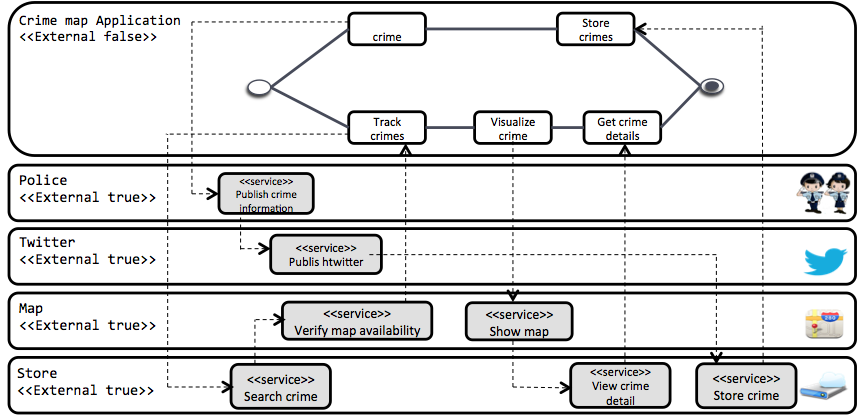
\includegraphics[width=0.95\textwidth]{figs/piServiceComposition}}
~ %add desired spacing between images, e. g. ~, \quad, \qquad etc. (or a blank line to force the subfig onto a new line)
\\
\subfloat[$\pi$-ServiceComposition Policies]
{\label{fig:crimePolicies}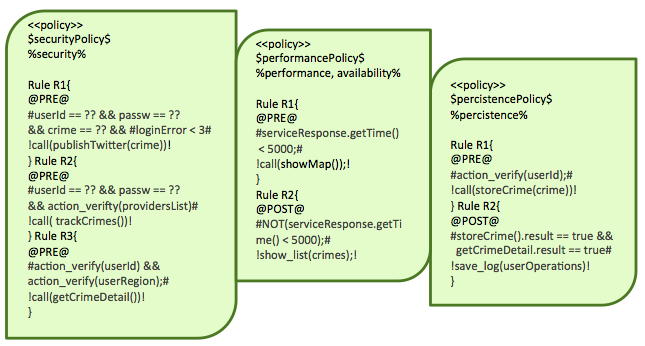
\includegraphics[width=0.85\textwidth]{figs/policies}}
~ %add desired spacing between images, e. g. ~, \quad, \qquad etc. (or a blank line to force the subfig onto a new line)
\caption{Service Composition and Policies.}
\label{fig:policies}
\end{figure}
This model describes the service compositions and their related business
collaborators (external services), policies, rules associated with a policy and
the whole application process and functionalities.
The workflow execution will consider the composition of business services and
their specific Business Collaborators. 
Each action will trigger the execution of one or more external services. 
Before and after each service call, policy rules are verified.

In the case of our crime tracking example, the model produced from the $\pi$-\textit{ServiceProcess} model of Figure~\ref{fig:piSP} is given in Figures~\ref{fig:piSC} and~\ref{fig:crimePolicies}.
Figure~\ref{fig:piSC} shows how the crime application interacts with its \textit{busines collaborators} (external services and entities).
The interaction occurs by means of function calls (denoted by dotted lines in the figure).
Figure~\ref{fig:crimePolicies} shows the definition of three \textit{policies}, which define rules for service execution.
In our case we have policies for \textit{Security}, \textit{Performance} and \textit{Persistence}. 


\paragraph*{$\pi$\textit{-PEWS} Model:}
These models are produced by a model-to-text transformation that takes a $\pi$-\textit{ServiceComposition} model and generates $\pi$-\textit{PEWS} specification code.
This code is a service composition program that can be compiled into executable code.
$\pi$-\textit{PEWS} models are expressed in a variant of the PEWS composition language.

\begin{figure}[t]
\footnotesize
%\begin{lstlisting}[label=list:rulePre,caption=ATL - piServiceComposition2piPEWS : Pre-condition Rule. ]
%\begin{lstlisting}[label=list:rulePre]
\begin{verbatim}
//Namespaces specify service URI
1 namespace twitter = www.twitter.com/service.wsdl
2 namespace googlemaps = maps.googleapis.com/maps/api/service
3 namespace amazondynamodb = rds.amazonaws.com/doc/2010-07-28/AmazonRDSv4.wsdl
4 namespace police = www.police.fr/service.wsdl

//Operations 
5 alias publishTwitter = portType/publishTwitter in twitter
6 alias searchCrime = portType/searchCrime in amazondynamodb 
7 alias showMap = portType/showMap in googlemaps 
...
//Services
8  service notifyCrime = publishCrime  . publishTwitter 
9  service trackCrime= searchCrime . verifyService
10 Service visualizeCrime =  showMap . getCrimeDetail
...
//Path
11 ( notifyCrime . storeiCrime ) || 
12 ( trackCrime . visualizeCrime . getCrimeDetail )
...
//Contracts
13 defContract notifyCrimeContract{
14	isAppliedTo: notifyCrime
15	requires: userId == ?? && passw == ?? && 
16	                               req(notifyCrime)  < 3
17 	  (OnFailureDo: NOT(action_publish(crime));
18	ensures: publishTwitter(crime) == true
19 	  (OnFailureDo: skip);
20 }
...
\end{verbatim}
% \end{lstlisting}
\caption{$\pi$-PEWS code for the crime tracking example (partial, simplified).\label{fig:pewscontract} }
\end{figure}

The $\pi$-PEWS program generated from the model in Figure~\ref{fig:policies} is partially presented in Figure~\ref{fig:pewscontract}. 
The figure shows a simplified program code, produced in accordance to the following guidelines:
\begin{trivlist}
\item[1.] Namespaces, identifying the addresses of external services are produced from the Business Collaborators of the higher-level model. 
We define four of them, corresponding to the Police, Twitter, Google Map and Amazon partners.
\item[2.] Specific operations exported by each business collaborator are identified to an \textit{operation} of the program (Each operation is given an \texttt{alias}).
\item[3.] The workflow in Figure~\ref{fig:piSC} is translated into a textual representation (lines 11 and 12 of the program).
\item[4.] \textit{Contracts} are defined in $\pi$-PEWS as having pre-conditions (\texttt{requires}), post-conditions (\texttt{ensures}) and actions (\texttt{OnFailureDo}) to be executed in the case thar a condition is not verified. 
Contracts are generated from Policies (such as those of Figure~\ref{fig:piSC}.
\end{trivlist}


For a more comprehensive account of $\pi$SOD-M the reader can refer to~\cite{SouzaNeto:2012}.

